% COMMON RINGS
\newcommand{\N}{\mathbb{N}}
\newcommand{\R}{\mathbb{R}}
\newcommand{\Z}{\mathbb{Z}}
\newcommand{\T}{\mathbb{T}}
\renewcommand{\S}{\mathbb{S}}

% Crossings and singularities
\newcommand*{\double}{\adjustbox{valign=c}{
\includegraphics[width=0.05\textwidth]{graphics/glyph_singular_point.pdf}}}
\newcommand*{\poscross}{\adjustbox{valign=c}{
\includegraphics[width=0.05\textwidth]{graphics/glyph_positive_crossing.pdf}}}
\newcommand*{\negcross}{\adjustbox{valign=c}{
\includegraphics[width=0.05\textwidth]{graphics/glyph_negative_crossing.pdf}}}

% T4T and T1T graphics
\newcommand*{\tftsouth}{\adjustbox{valign=c}{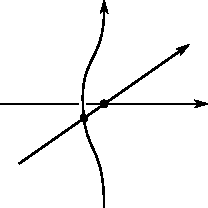
\includegraphics[width=0.11\textwidth]{topological_four_term_south.pdf}}}
\newcommand*{\tfteast}{\adjustbox{valign=c}{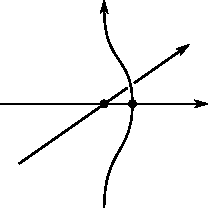
\includegraphics[width=0.11\textwidth]{topological_four_term_east.pdf}}}
\newcommand*{\tftnorth}{\adjustbox{valign=c}{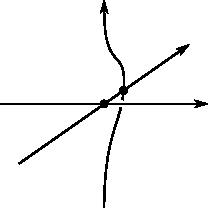
\includegraphics[width=0.11\textwidth]{topological_four_term_north.pdf}}}
\newcommand*{\tftwest}{\adjustbox{valign=c}{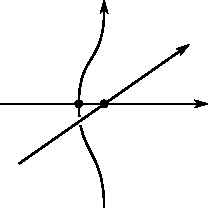
\includegraphics[width=0.11\textwidth]{topological_four_term_west.pdf}}}

\newcommand*{\totgraphic}{\adjustbox{valign=c}{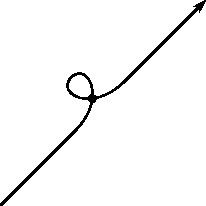
\includegraphics[width=0.11\textwidth]{topological_one_term.pdf}}}

% T4T and T1T (as sums of singular knots)
\newcommand{\tftterm}{\mathbf{T4T}}
\newcommand{\totterm}{\mathbf{T1T}}

% T4T and T1T, DIFF (as relations on invariants)
\newcommand{\tft}{\texttt{T4T}}
\newcommand{\tot}{\texttt{T1T}}
\newcommand{\diff}{\texttt{DIFF}}

% T4T and T1T, DIFF (as relations on singular knots)
\newcommand{\tftdual}{\texttt{T4T}\ensuremath{^\ast}}
\newcommand{\totdual}{\texttt{T1T}\ensuremath{^\ast}}
\newcommand{\diffdual}{\texttt{DIFF}\ensuremath{^\ast}}

% 4T and 1T graphics
\newcommand*{\ftsouth}{\adjustbox{valign=c}{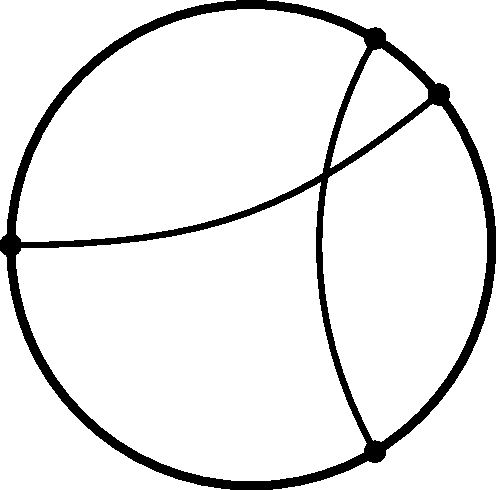
\includegraphics[width=0.11\textwidth]{four_term_south.pdf}}}
\newcommand*{\fteast}{\adjustbox{valign=c}{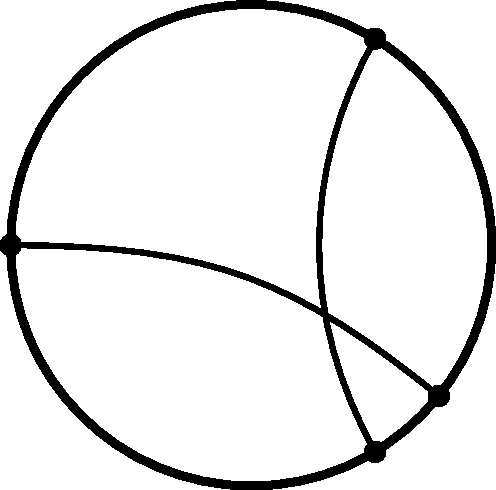
\includegraphics[width=0.11\textwidth]{four_term_east.pdf}}}
\newcommand*{\ftnorth}{\adjustbox{valign=c}{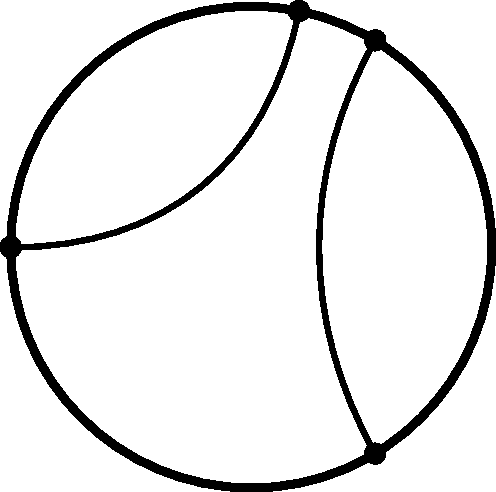
\includegraphics[width=0.11\textwidth]{four_term_north.pdf}}}
\newcommand*{\ftwest}{\adjustbox{valign=c}{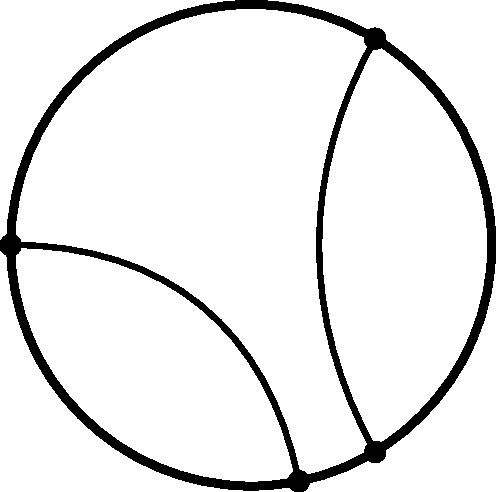
\includegraphics[width=0.11\textwidth]{four_term_west.pdf}}}

\newcommand*{\otgraphic}{\adjustbox{valign=c}{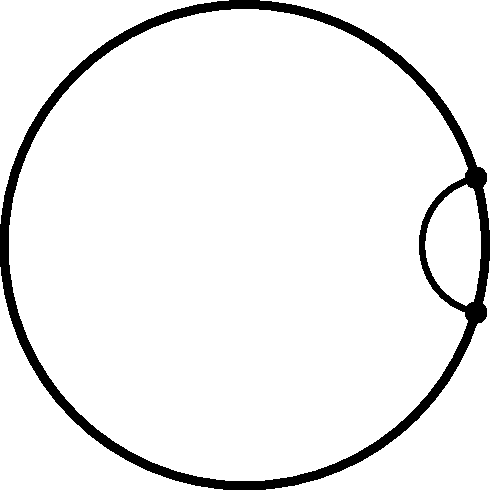
\includegraphics[width=0.11\textwidth]{one-term.pdf}}}

% 4T and 1T (as relations on constants of integration)
\newcommand{\ft}{\texttt{4T}}
\newcommand{\ot}{\texttt{1T}}

% 4T and 1T, DIFF (as relations on chord diagrams)
\newcommand{\ftdual}{\texttt{4T}\ensuremath{^\ast}}
\newcommand{\otrel}{\texttt{1T}\ensuremath{^\ast}}

